\section{État de Glasir à la conclusion du projet}
\label{sec:etatFinal}

Cette section va présenter l'état dans lequel Glasir a été livré à l'issue du projet. Va être présenté un récapitulatif des objectifs initiaux et leur état d'achèvement dans la {\sc sous-section}~\ref{subsec:objOK}, avant d'évoquer en {\sc sous-section}~\ref{subsec:encorePlusMieux} des améliorations à envisager.

\subsection{Tenue des objectifs}
\label{subsec:objOK}

Cette section a pour rôle de récapituler d'abord les accomplissements relatifs à Glasir avant de mettre en évidence ceux concernant ADTool.

\subsubsection{Glasir}
\label{sssec:obj_glasir}

L'objectif du projet était de fournir à des experts en sécurité, familiers avec le formalisme des ADTrees, une solution logicielle pour analyser et exploiter ces derniers. L'utilisation de cette solution logicielle, Glasir, devait se faire au moyen d'un ensemble de \og{modules}\fg constituant les fonctionnalités d'analyse des ADTrees, au sein d'une interface graphique simple et claire.

    \begin{figure}[!h]
        \centering
        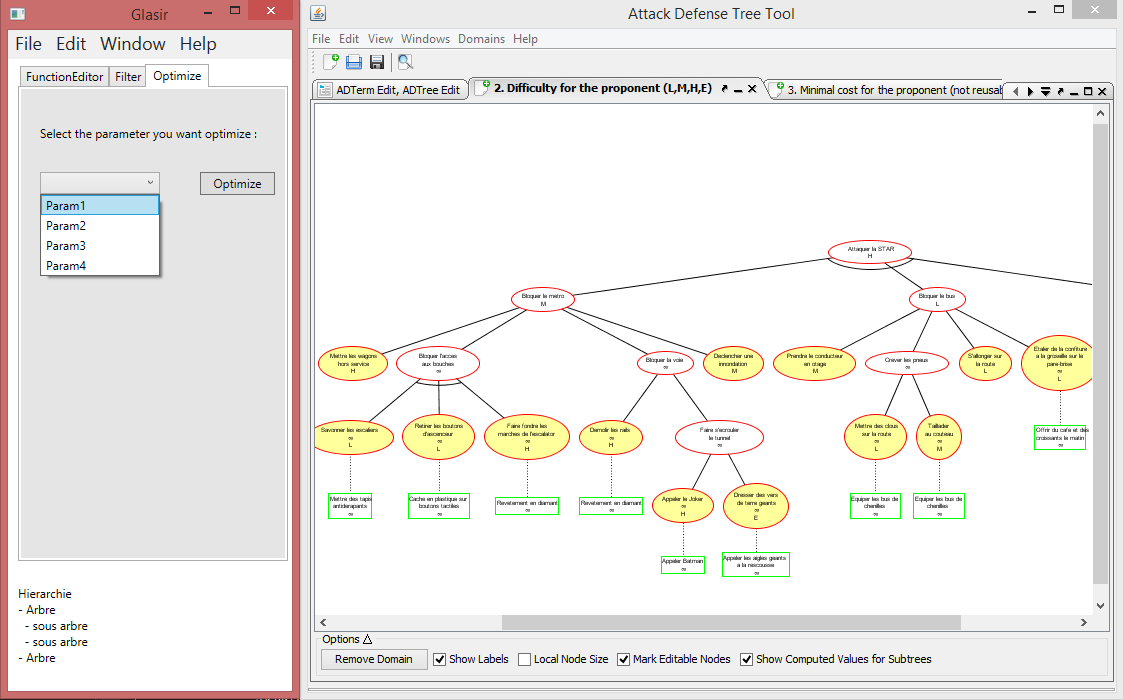
\includegraphics[height=0.5\textwidth]{figure/interface.png}
        \caption{Interface du logiciel Glasir.}
        \label{fig:InterfaceGlasir}
    \end{figure}

L'interface graphique de Glasir a été correctement implémentée avec les éléments qui avaient été promis : 
\begin{itemize}
	\item les trois fonctionnalités principales bien mises en évidence ;
	\item les ADTrees contenus dans le projet en cours ;
	\item un menu intuitif pour l'utilisateur.
\end{itemize}
Le seul écart à noter est qu'ADTool n'est finalement pas complètement intégré à Glasir. Les deux logiciels, bien que liés, restent indépendants dans le sens où bien que Glasir ait besoin de et utilise ADTool pour fonctionner, il ne communique pas avec ce dernier. Les éventuels soucis de cohérence des ADTrees entre les deux logiciels à la suite de modifications, induits par l'indépendance de ADTool et Glasir, ont été contournés grâce à la mise en place d'un \og view mode \fg{} pour ADTool, comme expliqué en détails dans la {\sc section}~\ref{sec:rect}. L'expérience utilisateur ne semble pas affectée par cette décision, qui permet en plus de mieux distinguer l'édition des ADTrees de leur analyse. Enfin, il sera joint à la version finale de Glasir un dossier faisant office de bibliothèque de modèles et contenant un certain nombre d'ADTrees pouvant être utilisés pour des tests mais aussi dans des projets. Ces ADTrees seront basés sur la thématique des transports en commun afin d'illustrer notre étude de cas sur le STAR (Service des Transports en commun de l'Agglomération Rennaise).

L'état des trois fonctionnalités principales de Glasir, qui confèrent au logiciel sont intérêt pour l'analyse, est détaillé dans les paragraphes suivants :

\paragraph{L'Éditeur de Fonctions} Ce dernier permet comme promis la combinaison de plusieurs paramètres, mais il est seulement possible d'en combiner deux en une seule fois. Cependant, il est ensuite possible de réutiliser les paramètres créés pour en produire de nouveaux, ce qui permet indirectement de combiner plus de deux paramètres. Les fonctions mathématiques utilisables sont comme annoncées les fonctions de base (somme, différence, produit, division), associées à des coefficients éventuels. Seules les fonctions min et max ne sont finalement pas applicables, car la façon d'écrire la fonction ne s'y prêtait finalement pas.

\paragraph{Le Filtre} Cette fonctionnalité permet comme prévu de filtrer un ADTree selon un paramètre sélectionné (qui peut être l'un des paramètres créés par le biais de l'Éditeur de Fonctions). L'ensemble des valeurs acceptées par le filtre est à préciser en fournissant une valeurs limite. Le filtre conservera alors les chemins de l'arbre étant meilleurs ou au moins aussi efficaces selon le paramètre choisi que la valeur limite. Cela dit, il est impossible de filtrer en une seule fois un ADTree selon plusieurs paramètres, contrairement à ce qui avait été annoncé dans le rapport de spécifications. Celui-ci peut malgré tout être fait en appliquant le Filtre consécutivement sur différents paramètres et valeurs limites, et ce jusqu'à obtenir le filtrage définitif souhaité.

\paragraph{L'Optimiseur} Comme annoncé, l'Optimiseur permet de conserver simplement le ou les chemins les plus efficaces selon le paramètre demandé. Pas de remarques particulières sur cette fonctionnalité.

Ainsi, malgré quelques changements par rapports à ce qui avait été annoncé lors de la phase de conception, Glasir est bien capable de remplir le rôle qui lui avait été fixé :  Il fournit à l'expert en sécurité des outils d'analyse efficaces et simples à l'utilisation.

\subsubsection{ADTool}
\label{sssec:obj_adtool}

Le cahier des charges prévoyait en plus de l'implémentation de Glasir un certain nombre de modifications à apporter à ADTool. Parmi ces dernières, toutes ont été correctement mises en place, à l'exception de l'affichage simultané de plusieurs paramètres sur les noeuds d'un même ADTree. Cette nouveauté a été abandonnée car elle nécessitait une charge de travail trop importante, comme déjà expliqué dans la {\sc section}~\ref{sec:rect}.

Le logiciel permet donc toujours de créer, d'afficher et d'éditer des ADTrees de façon simple et intuitive, mais son ergonomie a été améliorée par les fonctionnalités suivantes :
\begin{itemize}
	\item une représentation textuelle des ADTrees plus complète ;
	\item la possibilité de copier-couper-coller des sous-arbre d'un ADTree ;
	\item l'annulation des actions précédentes.
\end{itemize}

Toutes les nouveautés évoquées ici apportent une réelle aide à l'expert en sécurité, qu'il veuille créer, éditer ou analyser des ADTrees. Mais notre logiciel peut encore être amélioré, c'est pourquoi la {\sc sous-section}~\ref{subsec:encorePlusMieux} présente une liste d'idées à creuser dans l'éventualité d'une continuation de l'implémentation.

\subsection{Améliorations possibles}
\label{subsec:encorePlusMieux}

Suite à nos recherches sur l'analyse des ADTree et à l'implémentation de Glasir, nous avons pu identifier des améliorations et de nouvelles fonctionnalités potentiellement utiles pour l'analyse des ADTrees. La liste d'améliorations proposées ci-après n'est évidemment pas exhaustive, elle présente juste quelques pistes qui pourraient être envisagées si le projet avait à être poursuivi.

\paragraph{Interconnectivité ADTool/Glasir} Sans parler d'intégrer totalement ADTool dans Glasir, il semble envisageable de trouver un moyen d'informer l'un des modifications effectuées via l'autre, et vice-versa. Il serait plus agréable pour l'utilisateur de pouvoir éditer et analyser les ADTrees à partir d'une même fenêtre logicielle, sans avoir à changer d'outil sans arrêt. Cette interconnectivité permettrait de se passer de la version \og view mode \fg{} d'ADTool actuellement utilisée dans Glasir. 

\paragraph{Suggestion de défenses} Un exemple d'un nouveau module d'analyse d'arbres qui nous a paru intéressant est celui de donner à Glasir un arbre représentant un système défendu, mais qui dans la réalité ne l'est pas. L'expert pourrait alors demander à Glasir, en lui ayant au préalable indiqué le coût de l'installation de chacune des défenses, de trouver la disposition idéale des défenses contre une attaque compte tenu d'un critère (par exemple le temps nécessaire à l'attaque, le prix de l'attaque), pour un budget donné.